\chapter{Study Annotations}
\label{chap:study-annotations}
Annotations allow a study to collect custom named and defined pieces of data
for participants, collection events, and specimen processing.  Annotations are
optional and are not required to be defined for a study. Figure
\ref{fig:study-annotations} show the possible annotations types that can be
configured for a study. Annotations types must be defined before they can be
assigned to the respective entity.

\begin{figure}[H]
  \centering
  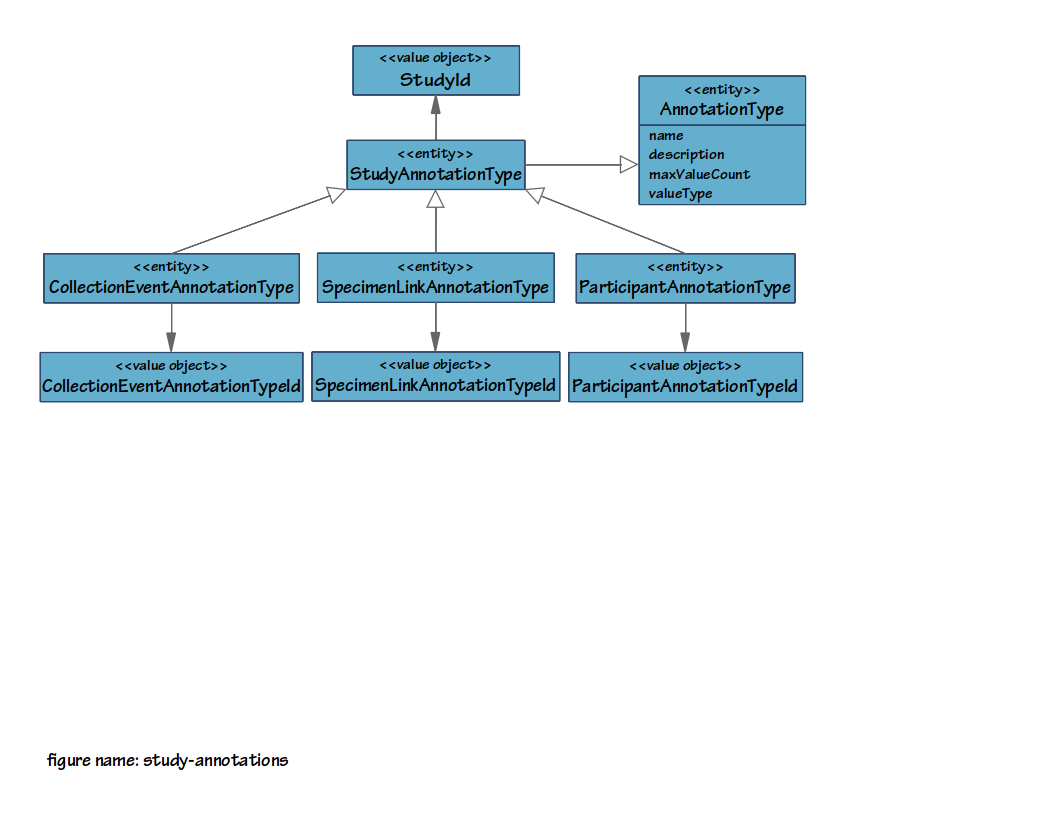
\includegraphics[trim={9mm 90mm 20mm 9mm}, clip,
    width=0.9\textwidth]{images/study-annotations}
  \caption{Study annotation entities}
  \label{fig:study-annotations}
\end{figure}

\subsection*{CollectionEventTypeAnnotationType}
A \entitytarget{CollectionEventTypeAnnotationType} is used to to configure an
annotation to be used by collection event types. An example of an annotation on
a collection even type can be consent given by the participant at the
collection visit.

\subsection*{SpecimenLinkAnnotationType}
A \valobjtarget{SpecimenLinkAnnotationType} is used to to configure an
annotation to be used with specimen link types.

An example of an annotation type on a specimen link can be the PMBC count on
the collected specimen.

\subsection*{ParticipantAnnotationType}
A \valobjtarget{ParticipantAnnotationType} is used to to configure a an
annotation for a participant.

An example of an annotation on a participant can be their gender.

\section{Participant Annotations Details}
Figure \ref{fig-participant-annotations} shows the annotation entities related
to participant annotations. The model used for annotations in collection event
and specimen processing is similar.

\begin{figure}[H]
  \centering
  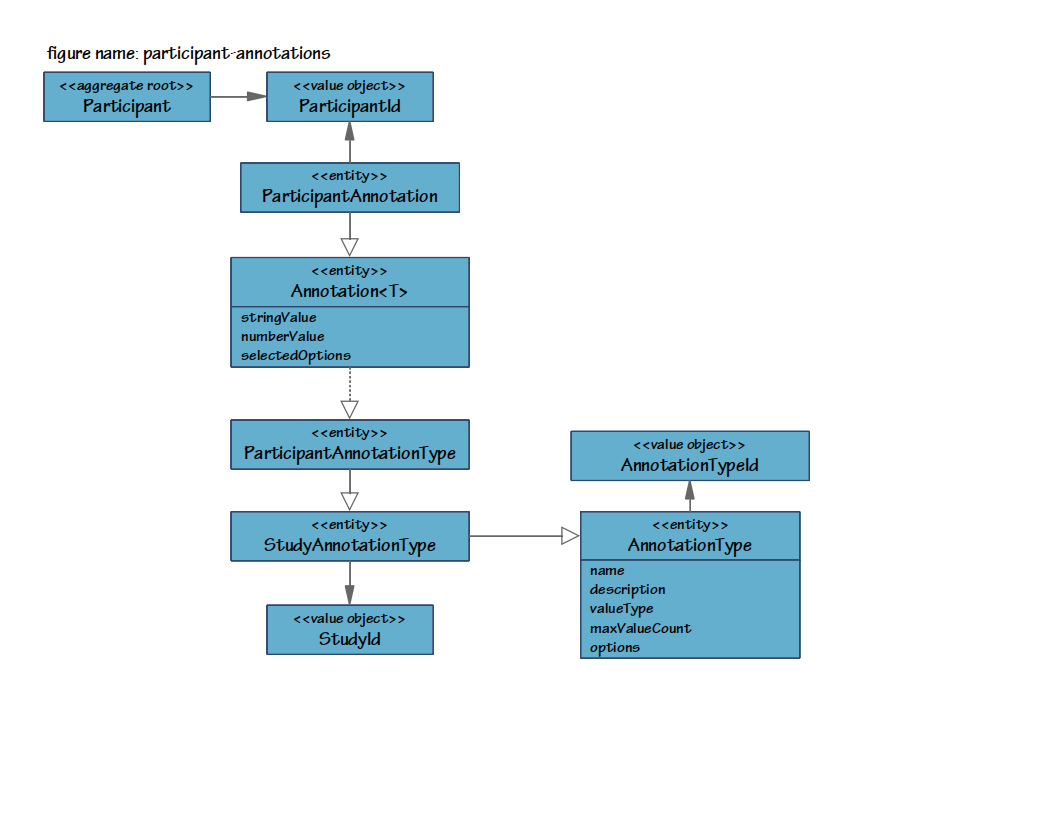
\includegraphics[trim={10mm 45mm 62mm 10mm}, clip,
    width=0.8\textwidth]{images/participant-annotations}
  \caption{Participant Annotations}
  \label{fig-participant-annotations}
\end{figure}

The \entitylink{ParticipantAnnotation} is a derived class of the generic class
\entitytarget{Annotation}. Possible annotations for a study are defined using
\entitylink{ParticipantAnnotationType} which is a derived class for
\entitylink{StudyAnnotationType} which itself is a derived class of
\entitytarget{AnnotationType}.

An annotation type has a short identifying name that is unique to the study. A
description can also be defined but is optional. The following table shows the
possible values for \compfont{valueType}. The value type specifies what the
annotation stores.

\begin{table}[H]
\renewcommand{\arraystretch}{1.1}
\begin{tabularx}{\textwidth}{@{\hspace{6pt}} >{\ttfamily}l X }
  \sffamily{\textbf{Value Type}} & \sffamily{\textbf{What is stored}}\\
  \hline

  String & an alphanumeric string.\\
  Number & a number, either integer or decimal.\\
  Date & date string, usually of the form \emph{YYYY-MM-DD HH:MM}.\\
  Select & a value selected from a predefined list.\\

\end{tabularx}
\end{table}

When \compfont{valueType} is assigned to be of type \compfont{Select},
\compfont{maxValueCount} is the number of of items that can be selected from the
predefined list. If only one value is allowed, then \compfont{maxValueCount} has
a value of 1. If an unlimited number of values are allowed then,
\compfont{maxValueCount} has a value of 0.

One or more \entitylink{AnnotationOption}s are used to create the predefined
list of select options.

Of the fields \compfont{stringValue}, \compfont{numberValue}, or
\compfont{selectedValue} in \entitytarget{Annotation}, only a single one is
used to store the annotation value. The remaining fields are
\compfont{null}. The field that is used is referred to as the \emph{Value
  Field}. The Value Field used depends on the value
\compfont{AnnotationType.valueType}.

\begin{table}[!htbp]
\renewcommand{\arraystretch}{1.1}
\begin{tabularx}{\textwidth}{@{\hspace{6pt}} >{\ttfamily}l l}
  \sffamily{\textbf{ValueType}} & \sffamily{\textbf{Value field}}\\
  \hline
  String & \compfont{stringValue}\\
  Number & \compfont{numberValue}\\
  Date & \compfont{numberValue} and stored as the number of seconds\\
  Select & \compfont{selectedValue}\\

\end{tabularx}
\end{table}

\section{Commands}

The commands for adding a \entitylink{CollectionEventTypeAnnotationType} are shown
here. The commands to add annotations to \entitylink{SpecimenLink} and
\entitylink{Participants} as similar to these commands but are not listed here.

See the \entitylink{AddCollectionEventTypeAnnotationOptions} command below for
adding annotation options to \compfont{SELECT} annotation types.

\subsection*{CreateCollectionEventTypeAnnotationType}

\begin{commandparmtable}
  studyId & String & The study's unique identifier.\\

  name & String & A short descriptive name.\\

  description & String & Provides more details. Can be left empty.\\

  valueType & \valobjlink{AnnotationValueType} & The types of values
  (e.g. string, number, date, etc.) this type of annotation expects.\\

  maxValueCount & Integer & If value type is \compfont{SELECT}, then this is the
  maximum number of selections that can be made. Use zero for unlimited.\\
\end{commandparmtable}

\subsection*{UpdateCollectionEventTypeAnnotationType}

\begin{commandparmtable}
  studyId & String & The study's unique identifier.\\

  collectionEventAnnotationTypeId & String & The annotation type's unique identifier.\\

  name & String & The updated or original name.\\

  description & String & The updated or original description.\\

  valueType & \valobjlink{AnnotationValueType} & The updated or original value type.\\

  maxValueCount & Integer & The updated or original count.\\
\end{commandparmtable}

\subsection*{DeleteCollectionEventTypeAnnotationType}

\begin{commandparmtable}
  studyId & String & The study's unique identifier.\\

  collectionEventAnnotationTypeId & String & The annotation type's unique identifier.\\
\end{commandparmtable}

\subsection*{AddCollectionEventTypeAnnotationOptions}
\hypertarget{AddCollectionEventTypeAnnotationOptions}{}

Adds annotation options for a \compfont{SELECT} annotation type.  The command
fails if the annotation value type is not \compfont{SELECT}.

\begin{commandparmtable}
  studyId & String & The study's unique identifier.\\

  collectionEventAnnotationTypeId & String & The annotation type's unique
  identifier.\\

  options & Set[String] & The options to add for this annotation.\\
\end{commandparmtable}

\subsection*{RemoveCollectionEventTypeAnnotationOptions}

Removes annotation options for a \compfont{SELECT} annotation type.  The command
fails if the annotation value type is not \compfont{SELECT}.

\begin{commandparmtable}
  studyId & String & The study's unique identifier.\\

  collectionEventAnnotationTypeId & String & The annotation type's unique
  identifier.\\

  values & Set[String] & A set containing strings for the values that should be
  removed.\\
\end{commandparmtable}

% Local Variables:
% compile-command: "/usr/bin/rubber --pdf main"
% End:



% Local Variables:
% compile-command: "/usr/bin/rubber --pdf main"
% End:
